\section{VoIP Standards}

Contrary to common belief VoIP is not a single protocol or protocol stack but a collection of technologies that maybe be assembled together to provide voice-like-data over the IP protocol. Simpler VoIP implementations concern themselves with the session and presentation layers of the OSI seven layer model, as illustrated. But when scaling this technology across enterprise or internet sized systems many deeper grained issues begin to appear such as fault tolerance, security, latency, mobility and quality of service.
\begin{center}
	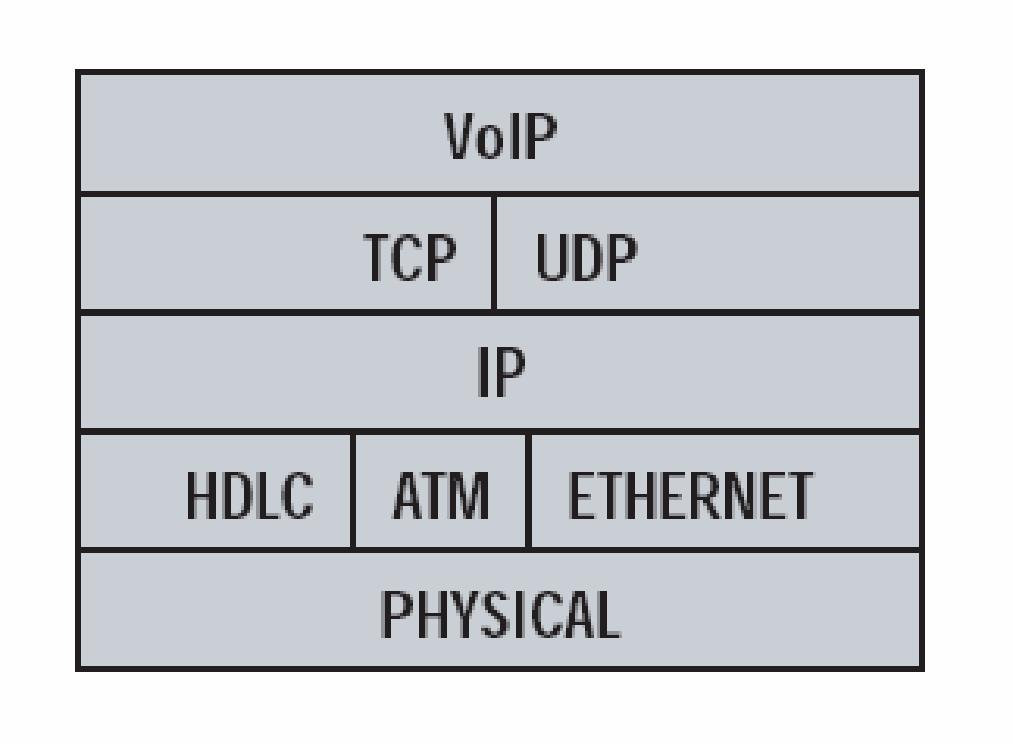
\includegraphics[width=2.5in]{images/simple_voip_protocol.jpg}
\end{center}

\subsection{H.323 - Packet-based multimedia communications systems}
A standard defined by the International Telecommunication Union (ITU) and was initially published in 1996\cite{website:itu_h323} the same month the SIP draft was published and was the first standards based VoIP stack\cite{website:packetizer_h323}. This standard encapsulates a number of ITU-T and IETF protocols used in the transmission of voice, video and data over a packet switched network.

The standard consists of a number of classes of components, below is a breakdown and description of these elements:

\begin{description}
\item[Terminals*] Voice and video handsets, high-definition videoconferencing systems, voicemail systems, softphones.
\item[Multipoint Control Units* (MCUs)] Responsible for managing multi-point conferences (two or more endpoints involved in  a conference).
\item[Gateways*] Interfaces to other networks e.g. PSTN, H.320 (VoIP using ISDN) or other H.323 networks (proxy).
\item[Gatekeeper] An optional component which manages admission control and address resolution and can be used to implement features such as follow-me/find-me or forward on busy.
\item[Border Elements and Peer Elements] Exchange addressing information and participate in authorisation across administrative domains. Peer elements are used to aggregate and reduce the volume of routing information exchanged across domains.
\end{description} 
*often referred to as endpoints

While all of the elements described above are not required, at minimum two terminals are required to facilitate communication between two people and in most deployments a gatekeeper is deployed to facilitate address resolution among other functions.

H.323 is described as a ‘framework’ document which defines how various protocols fit together. Common implementations of this standard may employ twelve or more protocols in to perform basic VoIP functionality. The standard covers all aspects of communication from T.120 for data conferencing to T.38 for fax transmission and from H.235 defining security to H.225.0 defining call signaling between endpoints.

From this brief overview of the standard it is quite clear to see that H.323 is a robust and complex standard defined by the telecommunications industry for the telecommunications industry. From its inception has been positioned as a ‘next generation’ to the POTS network offering voice, video, data, conferencing, roaming and other features naively while maintaining compatibility with legacy systems by way of support for PSTN numbering for example.

One criticism of this standard is its complexity due to its rigid specification for areas of the standard, which has slowed the deployment of these H.323 networks.

\subsection{SIP - Session Initiation Protocol}
The initial SIP draft document was published during the same period as the first revision of the H.323 standard was published in 1996. The SIP signaling protocol is published by a working group of the IETF (Internet Engineering Task Force), and due to this affiliation the standard relies much more heavily on existing internet protocols such as HTTP, in contrast H.323 utilises ISDN Q.931 protocol for signaling as well as numerous other telecommunication industry protocols.

SIP is regarded as a much simpler protocol when compared to H.323\cite{paper:miroslavvozna}, while maintaining a somewhat similar feature set\cite{paper:SchulzrinnRosenber} when communicating over IP.  The IETF approach to telephony signaling reuses many mechanisms from HTTP including authentication, encoding and error codes.

\begin{center}
	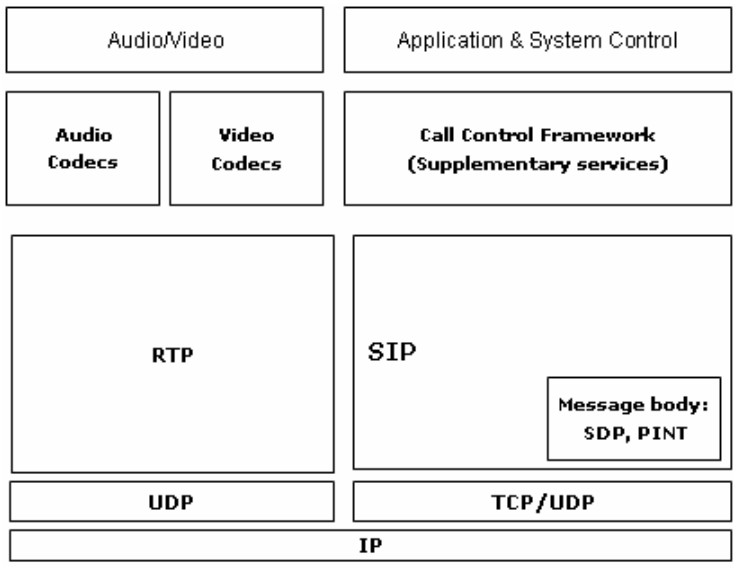
\includegraphics[width=3in]{images/sip_protocol_suite.png}
\end{center}

SIP was designed to control unicast or multicast multimedia communication sessions over IP, example applications of the protocol would include voice and video streaming, conferencing, online gaming and instant messaging to name a few.

The protocol is only involved in the signaling portion of a VoIP session, the design of the protocol borrows many elements from the HTTP protocol, utilising its request/response model and the packet header is largely the same. For the transmission most typically UDP or TCP are used to connect to other SIP endpoints and encryption is provided utilising TLS (Transaction Layer Security) the same mechanism used to secure HTTP transactions.

Unlike H.323 the design goal of SIP was to provide a signaling and call setup protocol and not to rigorously define all the potential features of the protocol, while offering expandability to offer features far beyond a traditional PSTN network. Depending on specific implementation SIP can be peer-to-peer, enabling the creation of a scalable and decentralised network.

Below you can see an example of the SIP architecture, communication is initiated using a SIP server but the actual media transmission is on a peer-to-peer basis, with only external lookups for authentication and authorisation.

\begin{center}
	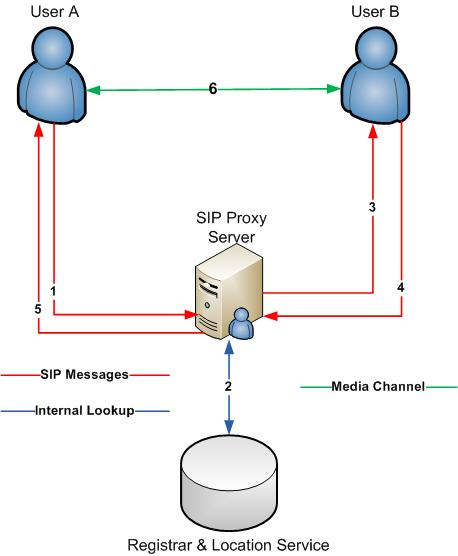
\includegraphics[width=3in]{images/SIP_Architecture.jpg}
\end{center}

Proponents of SIP distinguish the protocol from existing VoIP protocols such as H.323 to SIP’s roots laying in IP and being governed by the IETF and not by the telecommunications industry. H.323 is the more mature standard at this point but lacks in flexibility, for example at does not support presence information. SIP appears to be gaining more deployments in the corporate environment, but has issues with interoperability due to vendor specific additions.

\subsection{Skype}
Skype unlike H.323 and SIP is a closed source propriety protocol, network and business model. Due to the nature of Skype much is unknown about the details of the protocol, but considering the usage numbers mentioned earlier in this paper omitting an overview of what is known about the Skype protocol would leave this document lacking.

The system is designed as a peer-to-peer network which allows the company to operate a small core network of login servers, reducing their bandwidth requirements and aiding in maintaining a high degree of uptime. The remainder of the network comprises of normal Skype clients, these clients have two operating modes node and super-node. Below is an architectural diagram of a Skype based network.

\begin{center}
	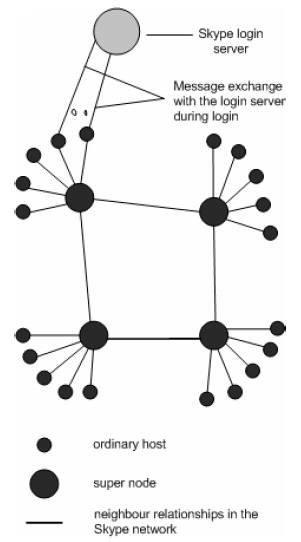
\includegraphics[width=2.5in]{images/Skype_network2.png}
\end{center}

Any node with a public IP address having sufficient CPU, memory, and network bandwidth is a candidate to become a super node\cite{website:BasetSchulzrinne}. These super nodes may relay communications for regular nodes located behind a NAT or Firewall configuration, which is a common issue for many peer-to-peer networks. For a regular node to connect to to the network it must register itself with the login servers and connect to a super-node.

With a peer-to-peer approach such as this authentication and privacy become important elements to the protocol. As we have already discussed all authentication is managed via the Skype central login servers, Skype ensures privacy in the channel between two or more communicating users by transparently encrypting the data stream. For this encryption the protocol uses RSA 1024bit for authentication, RC4 for signaling and 256bit AES for VoIP, offering the user a quite reasonable level of security\cite{website:Fabrice05}. 

Skype recently submitted their Skype SILK wideband audio codec to the IETF for standardisation\cite{website:IETFSILK10}, but the protocol is also believed to use G.729 and SVOPC in transmission of audio. For video transmission it is believed that Skype utilise VP7 from On2 Technologies, but since Google’s acquisition of the company and the removal of their website its impossible to confirm this.

While the Skype protocol may not be as all encompassing as H.323 and SIP it feature set is large enough to be positioned as a viable VoIP alternative. It has support for voice, video, data and text messaging as well as conferencing, mobile usage and presence information. And offering an interesting third architectural option for a VoIP implementation.

